\chapter{Gezondheidsapplicatie}
Voorgaand onderzoek met betrekking tot herkenning van rope skipping bewegingen zal in wat volgt geïntegreerd worden in een gezondheidsapplicatie.
Met dit systeem is het de bedoeling dat de gebruiker via zijn/haar smartwatch sessies kan starten waarvan nadien statistieken weergegeven worden op de bijhorende smartphone applicatie. Hierbij wordt gefocust op rope skipping. Data processing van rope skipping zal gebeuren aan de hand van een eigen model (zie hoofdstuk \ref{chapter:3}). Een sessie rope skipping zal meer info geven aan de gebruiker in de vorm van tijdstippen met betrekking tot uitgevoerde bewegingen, het aantal draaiingen en eventuele geregistreerde tekortkomingen. Het is de bedoeling dat, gebaseerd op deze data, persoonlijke aanbevelingen gegeven worden. Alle informatie wordt, op basis van het id afkomstig van het Google account waarmee ingelogd werd, opgeslagen in een SQLite database. Dit gedeelte van het onderzoek werd uitgewerkt aan de hand van een voorgaande thesis \cite{ref73}. Hieruit werden ideeën opgedaan om vervolgens een eigen systeem te ontwikkelen.

\section{Backend - Frontend}
Het model werd getraind in Python. Er moet nu een afweging gemaakt worden tussen behouden van de scheiding van backend en frontend of migreren van de backend naar de frontend. Beide opties hebben voordelen en nadelen. Laten we eerst kijken naar de backend - frontend optie. Hierbij kan de code in Python behouden worden. Python is namelijk zeer efficiënt om aan data analyse te doen. Het beschikt over handige libraries zoals Pandas waarmee data door middel van reeds geïmplementeerde functionaliteit kan bewerkt worden. De server waarop de backend zou draaien heeft ook meer rekenkracht dan een android smartphone of smartwatch. Hierdoor kunnen zwaardere maar accuratere machine learning methodes gebruikt worden. Er is echter wel constant internetconnectie nodig om recente updates te krijgen.
Een louter frontend aanpak zal het probleem van offline werken aanpakken. De berekeningen worden nu op de applicatie zelf uitgevoerd. De resultaten zijn dus meteen beschikbaar voor de gebruiker. Een android smartphone heeft echter minder rekencapaciteit (alhoewel dit vandaag de dag nog meevalt) waardoor zeer zware berekeningen niet mogelijk zijn. Ook is het minder intuïtief om in Java aan data analyse te doen. 
Er werd gekozen voor de frontend aanpak. Dit omdat het belangrijk is meteen na een sessie statistieken weer te geven. Op die manier wordt voor optimale mentale stimulatie gezorgd. Zoals eerder vermeld, zijn hedendaagse android smartphones geschikt om zwaardere taken te draaien. Deze frontend aanpak is bijgevolg verantwoord. 

\section{Android opslag}
De applicatie zal aan de hand van vier Tensorflow Lite modellen online voorspellingen uitvoeren. Deze modellen moeten bijgevolg toegankelijk zijn voor de applicatie. Hierbij moet een keuze gemaakt worden tussen inwendig en uitwendig geheugen. Voor elke applicatie wordt bij opstarten een map voorzien in het inwendig geheugen. Hierin wordt gevoelige applicatie specifieke data opgeslagen en is bijgevolg niet toegankelijk voor andere applicaties. Het uitwendig geheugen daarentegen is toegankelijk voor elke applicatie. Ook is de beschikbare ruimte groter in vergelijking met het inwendig geheugen. Data opgeslagen in het uitwendig geheugen is echter minder betrouwbaar. De gebruiker kan namelijk elk moment beslissen om het geheugen te verwijderen \cite{ref75}. Om deze reden werd gekozen voor opslag in het inwendig geheugen.

\section{Smartwatch applicatie}
De smartwatch applicatie staat in voor het starten van sessies en het verzamelen van data tijdens deze sessies. De accelerometer en hartslag datapunten worden via de MessageClient API verstuurd naar de android applicatie draaiende op een smartphone. Aangezien aan een frequentie van 52Hz gemeten wordt, kan versturen van datapunten in realtime een invloed hebben op de batterijlevensduur en/of performantie van de applicatie. Om deze redenen wordt gekozen voor het verzenden van de data in batches van 104 datapunten. Voor de verzameling van hartslagdata moet de gebruiker eerst toestemming geven. De body sensors permissie wordt bestempeld als een zogenaamd gevaarlijke permissie waardoor deze \textit{at runtime} moet toegekend worden. 
De gebruiker wordt bij het starten van een sessie gevraagd om de corresponderende smartphone te selecteren. Indien deze niet in de lijst te vinden is, wordt gevraagd om bluetooth in te schakelen (zie Figuur \ref{fig:bluetooth}).
Tijdens een sessie wordt eveneens de hartslag gemonitord (zie Figuur \ref{fig:session}), indien deze gevaarlijk hoog wordt zal de smartwatch dit signaleren via een trilling. Hiervoor is extra informatie nodig. De maximum hartslag wordt namelijk berekend op basis van de leeftijd. Om deze reden zal, wanneer het startsignaal verstuurd wordt, een bericht met als inhoud de ingestelde leeftijd verkregen worden afkomstig van de smartphone applicatie.

\begin{figure}[!htpd]
\centering
\begin{floatrow}
  \ffigbox[\FBwidth]{\caption{Smartwatch session}\label{fig:session}}{%
    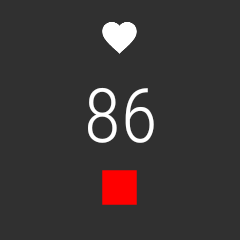
\includegraphics[width=.35\textwidth]{gezondheidsapplicatie/smartwatch-session.png}
  }
  \ffigbox[\FBwidth]{\caption{Smartwatch bluetooth}\label{fig:bluetooth}}{%
     
\includegraphics[width=.35\textwidth]{gezondheidsapplicatie/smartwatch-bluetooth.png}
  }
\end{floatrow}
\end{figure}

\section{Smartphone applicatie}
De smartphone applicatie staat in voor het ontvangen van datapunten en de verwerking hiervan. Het machine learning model is lokaal beschikbaar en wordt dan ook gebruikt om bewegingen te herkennen in de ontvangen accelerometer data. Ook worden het aantal draaiingen en eventuele fouten berekend. Per beweging zal het aantal MET-minuten (zie subsectie \ref{subsection:inspanningspunten}) berekend worden aan de hand van hartslag datapunten binnen een tijdsinterval bepaald door de duur van een sessie. Deze worden later gebruikt om aanbevelingen te genereren. 
Via een tijdlijn kan de gebruiker per sessie zien welke sprongen uitgevoerd werden (zie Figuur \ref{fig:tijdlijn}).
Elke week zullen de aanbevelingen berekend worden aan de hand van historische data. Deze zijn te zien op de applicatie zodat de gebruiker zelf kan kiezen wanneer hij/zij een aanbevolen activiteit uitvoert. Een aanbeveling kan omgezet worden in een effectieve sessie. Door een bericht te versturen via de MessageClient API naar de gekoppelde smartwatch wordt deze sessie gestart. De gebruiker wordt vervolgens gevraagd om de gewenste ontvanger te selecteren. Dit zodat geen problemen kunnen ondervonden worden indien meerdere bluetooth apparaten in de buurt aanwezig zijn (zie Figuur \ref{fig:bluetooth-phone}). De bijhorende aanbeveling wordt op \textit{pending} gezet zodat kan nagegaan worden of de gebruiker deze effectief uitvoert. Er wordt gecheckt of de duur van de activiteit overeenkomt met de aanbevolen duur en of het inspanningsniveau min of meer gelijklopend is.
Een afgewerkte aanbeveling wordt op \textit{done} gezet en uitgegrijsd weergegeven in de applicatie (zie Figuur \ref{fig:pending}).

\begin{figure}[!htpd]
\centering
\begin{floatrow}
  \ffigbox[\FBwidth]{\caption{Pending aanbevelingen}\label{fig:pending}}{%
    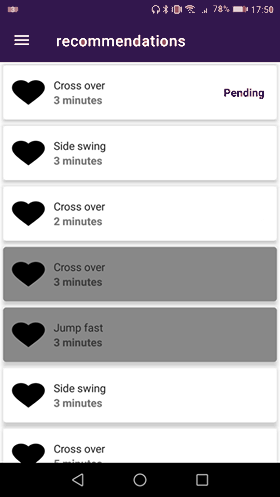
\includegraphics[width=.33\textwidth]{gezondheidsapplicatie/pending_recommendations.png} 
  }
  \ffigbox[\FBwidth]{\caption{Tijdlijn activiteiten}\label{fig:tijdlijn}}{%
    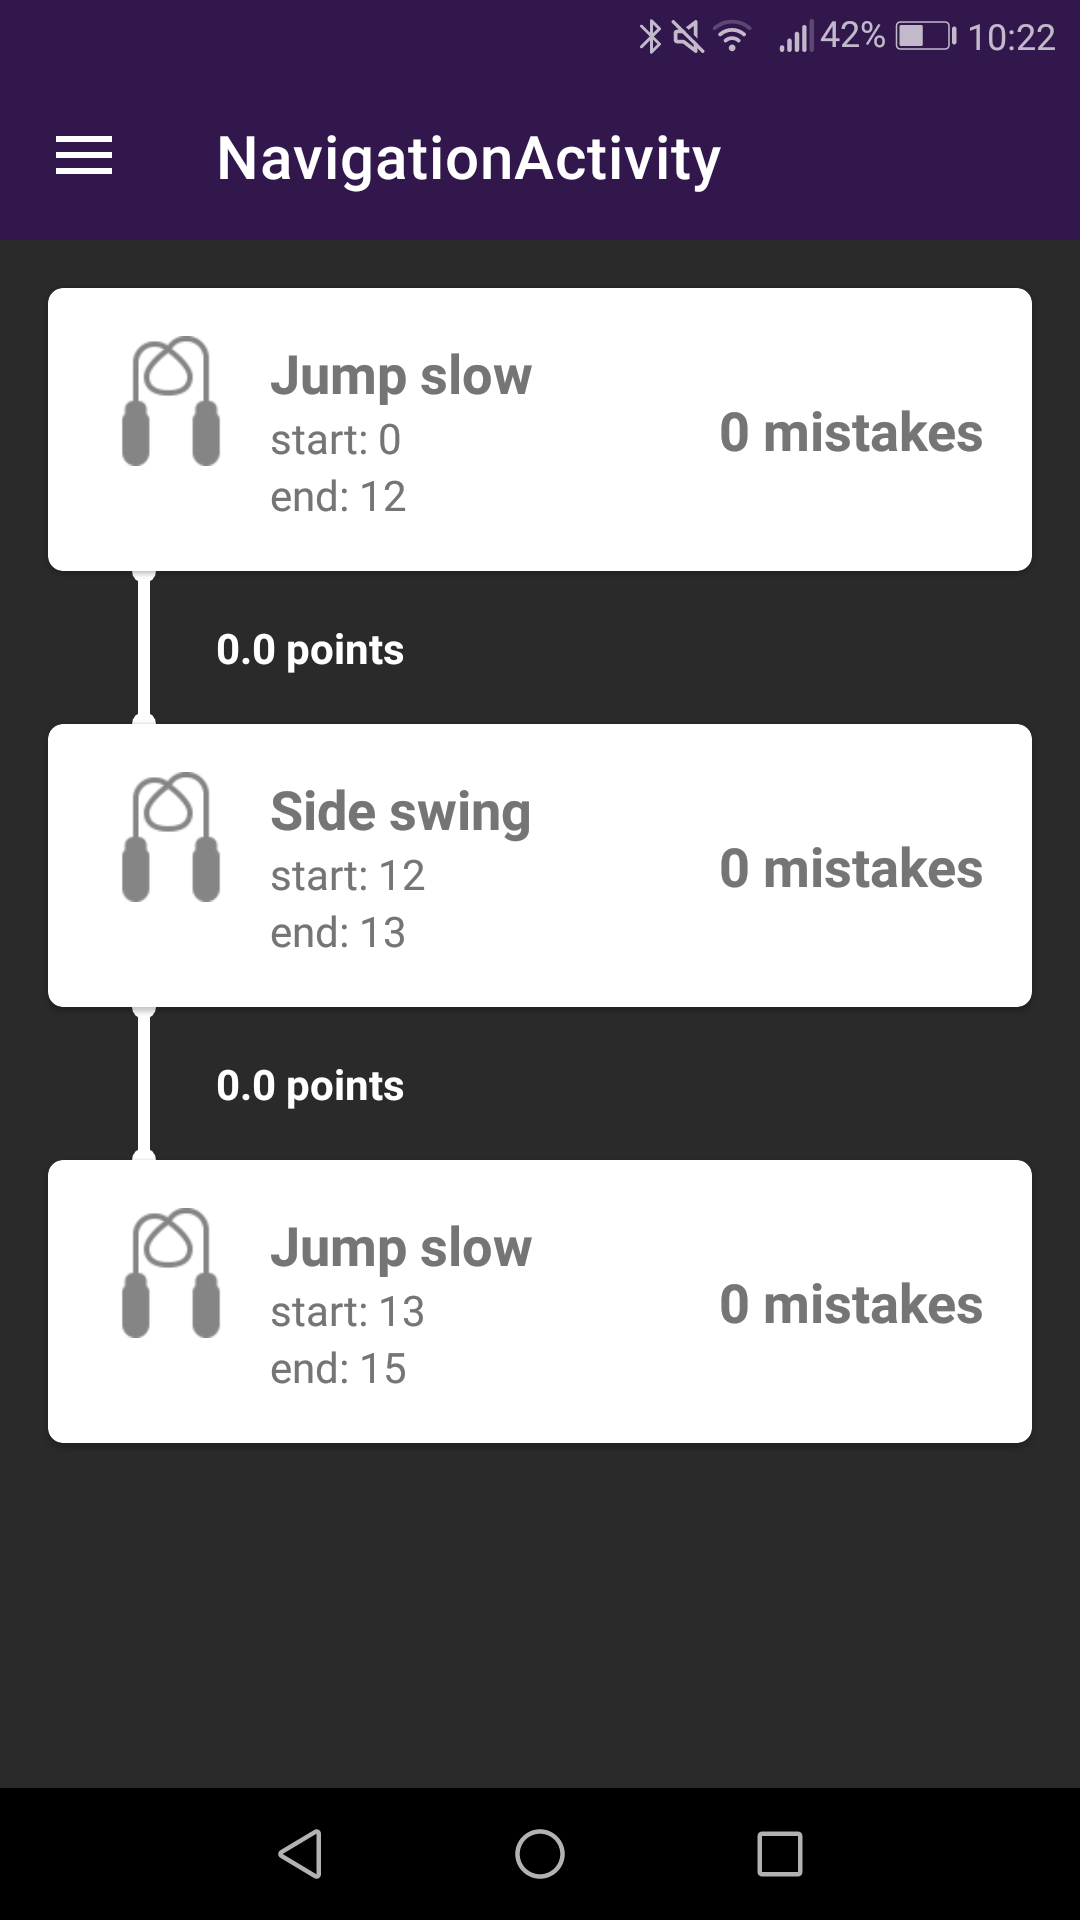
\includegraphics[width=.33\textwidth]{gezondheidsapplicatie/timeline.png} 
  }
  \ffigbox[\FBwidth]{\caption{Bluetooth dialog}\label{fig:bluetooth-phone}}{%
     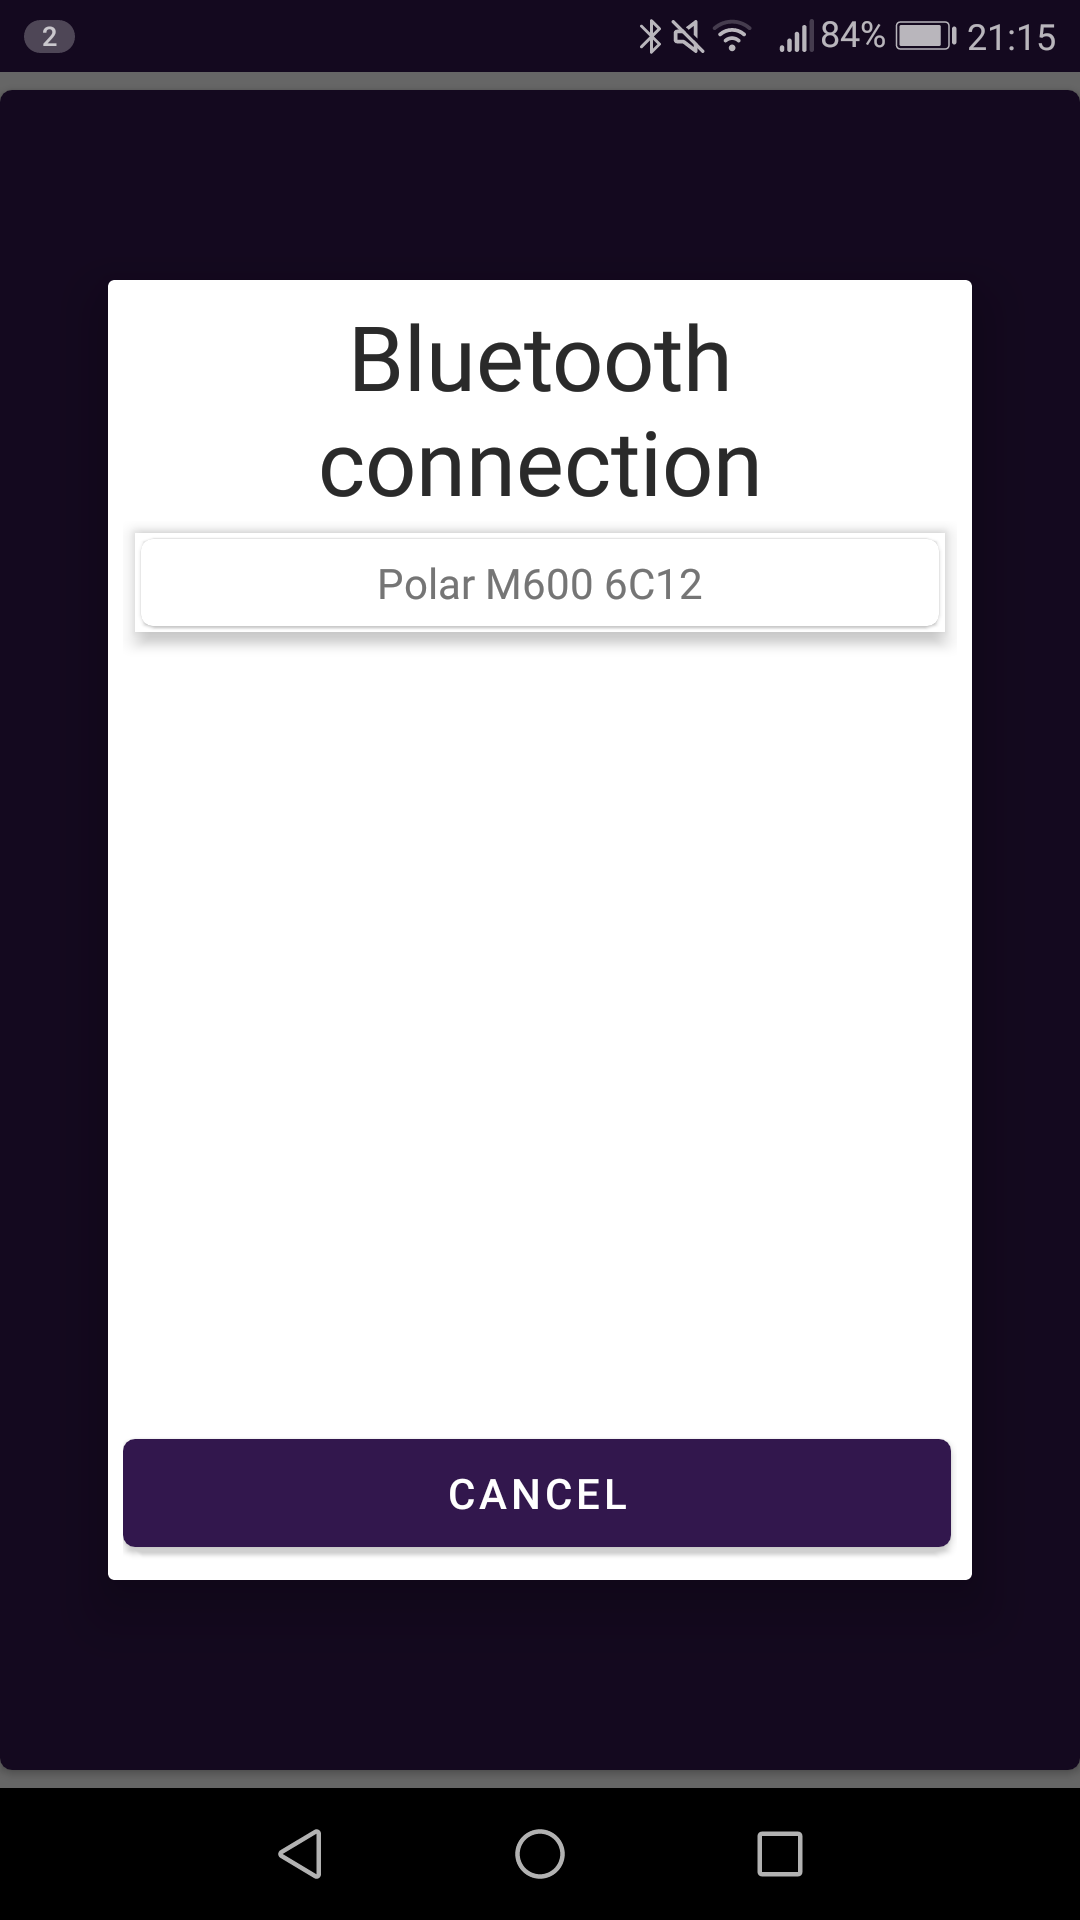
\includegraphics[width=.33\textwidth]{gezondheidsapplicatie/bluetooth_dialog.png} 
  }
\end{floatrow}
\end{figure}


\subsection{Aanbevelingen}
In deze subsectie worden eerst bestaande aanbevelingssystemen toegelicht. Vervolgens wordt het gebruikte aanbevelingsalgoritme besproken.

Een aanbevelingssysteem houdt rekening met de gebruiker en item dimensies.Er zijn verschillende manieren waarop dit kan geïmplementeerd worden.
Een eerste manier, Collaborative Filtering, bekijkt enkel interacties tussen gebruiker en item. Deze worden opgeslagen in een gebruiker-item interactie matrix. Verdere onderverdeling in een geheugen gebaseerde en een model gebaseerde aanpak is mogelijk. 

Een geheugen gebaseerde aanpak veronderstelt afwezigheid van een model en maakt in essentie gebruik van Nearest Neighbors. De items gekoppeld aan de gebruikers die het dichtst liggen worden aanbevolen. Ook hier kan nog eens een onderverdeling gemaakt worden in gebruiker-gebruiker en item-item.
Een gebruiker-gebruiker methode gaat gebruikers proberen identificeren met het meest gelijkaardige interactie profiel om zo nieuwe items aan te bevelen. Hierbij staat de gebruiker centraal. Gebruikers worden voorgesteld met een vector van hun interacties met items.
Een item-item methode gaat items zoeken gelijkaardig aan deze waarmee de gebruiker al positieve interactie mee had. Items worden gezien als gelijkaardig indien de twee gebruikers er op een gelijkaardige manier mee interageerden. Deze manier is bijgevolg gecentreerd rond het item.

Wanneer een model aanwezig is dan is er een zekere relatie tussen gebruiker en de gekoppelde items. Deze relatie wordt vervolgens gehanteerd bij voorspellingen.

Collaborative Filtering heeft als voordeel dat geen additionele info nodig is over gebruikers of items en kan dus in vele situaties gebuikt worden. Aanbevelingen worden ook accurater naarmate de gebruikers meer intrageren met items. Een nadeel is het cold start probleem. Dit doet zich voor door het feit dat enkel historische data bekeken wordt. Een nieuw item aanbevelen is onmogelijk en aan een nieuwe gebruiker kan niks aanbevolen worden. 

Content gebaseerde methoden gebruiken bijkomende info over de gebruiker en/of item objecten. Deze worden behandeld als features en kunnen helpen in verklaren waarom er juist een relatie is tussen die gebruiker en item. Deze methoden hebben geen last van cold start aangezien informatie altijd aanwezig zal zijn (leeftijd, geslacht..). Enkel nieuwe gebruikers of items met voorheen onbekende features ondervinden enige hinder.

Content gebaseerde methoden vervormen het probleem naar een classificatie of regressie probleem.
Indien de classificatie gebaseerd is op gebruikersfeatures dan wordt het item centraal geplaatst aangezien de berekeningen per item gebeuren.
Indien de classificatie echter op basis van item features wordt uitgevoerd dan is het algoritme gebruiker gecentreerd. Deze manier is persoonlijker omdat geen gebruik gemaakt wordt van data afkomstig van alle gebruikers. Het model is echter minder robuust vermits slechts één gebruiker met minder items interageerd \cite{ref50}.

Het systeem ontwikkeld tijdens deze thesis legt de nadruk vooral op het persoonlijke aspect. Daarom wordt gekozen voor een content gebaseerde methode gecentreerd rond de gebruiker. Het nadeel bij deze methode is hier ook niet echt van toepassing. Er zijn slechts een beperkt aantal bewegingen. De kans is dus groot dat 1 gebruiker deze allemaal uitvoert. Er zal echter wel enige hinder ondervonden worden door cold start. Van een nieuwe gebruiker is nog geen info geweten. Daarom worden een aantal willekeurige aanbevelingen gegenereerd zodat het systeem op termijn hieruit kan leren.

Elke week zal een nieuwe reeks aanbevelingen berekend worden. Hier wordt gebruik gemaakt van een PeriodicWorkRequest (zie subsectie \ref{subsection:workmanager}). Het ontwikkelde algoritme houdt rekening met het aantal sessies waarin een bepaalde activiteit uitgevoerd werd. Ook wordt het aantal fouten gemaakt tijdens een beweging in rekening gebracht. Er wordt gewerkt met een systeem dat gewichten toekent aan iedere activiteit op basis van eerder genoemde criteria. De duur van een aanbeveling wordt gelijkgesteld aan de gemiddelde duur van de gekozen activiteit op basis van historische data. Het totaal aantal MET-minuten van alle berekende aanbevelingen samen moet gelijk of groter zijn dan het doel gekoppeld aan die week. Dit totaal aantal METs wordt bekomen door gebruik te maken van het gemiddeld aantal METs per seconde voor iedere corresponderende activiteit en deze telkens op te tellen.
Indien nog geen sessies aanwezig zijn, dan kan nog geen rekening gehouden worden met de capaciteiten en voorkeuren van de gebruiker. Er wordt aan elke activiteit een gelijk gewicht toegekend. Om dezelfde reden wordt de duur van een activiteit willekeurig gekozen binnen het interval van 5 tot 10 minuten. Dit bleek een acceptabele duur te zijn voor beginnend rope skippers na enige rondvraging. Het is namelijk belangrijk om de initiële duur van de willekeurige aanbevelingen niet te groot te nemen. Een amateur rope skipper zou door een overschatting van zijn/haar capaciteiten al dan niet ontmoedigd worden. Het initiële doel wordt ingesteld op de gezonde waarde van 600 MET-minuten per week \cite{ref21}.
Een visualisatie van het ontwikkelde algoritme is te zien op Figuur \ref{fig:algo}.

\begin{figure}[!htpd]
\centering
\caption{Aanbevelingsalgoritme}\label{fig:algo}
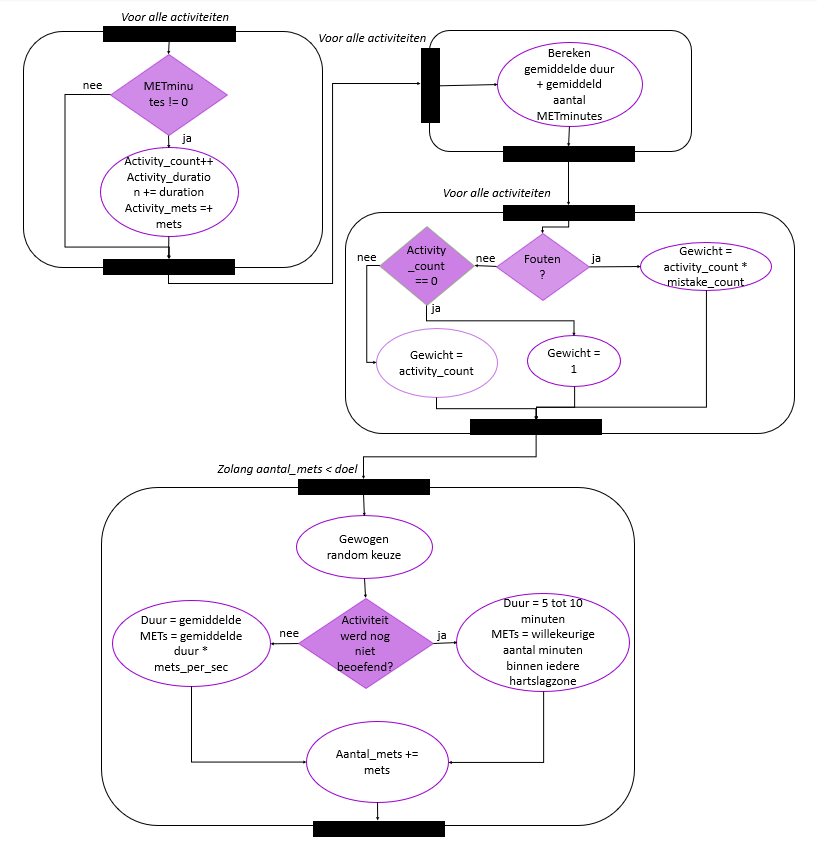
\includegraphics[width=1.15\textwidth]{gezondheidsapplicatie/recommendation_algo.PNG} 
\end{figure}

\subsection{Inspanningspunten} \label{subsection:inspanningspunten}
Het geven van persoonlijke aanbeveling steunt op een scoringmechanisme. De gebruikte metriek moet de mate van inspanning per activiteit correct weergeven. De MET-eenheid is hiervoor uitermate geschikt \cite{ref21}. Volgende paragrafen verduidelijken deze term.
De hoeveelheid energie die gebruikt wordt tijdens een inspanning is proportioneel tot de hoeveelheid zuurstof in het lichaam. Het aantal METs geeft hierbij de hoeveelheid zuurstof weer in geval van rust. De energie gevraagd van een fysieke activiteit kan uitgedrukt worden als een veelvoud van deze \textit{resting metabolic rate}. Dit is de Metabolic Equivalent of Task (MET). Een individu met gemiddelde fitness capaciteiten kan tot 12 METs verdragen, top atleten kunnen echter tot 20 aan. 
Een manier om het inspanningsniveau en dus het aantal METs te meten, is via de hoeveelheid zuurstof inname. Het zuurstofgehalte meten moet gebeuren aan de hand van strikte protocollen binnen een sport laboratorium. Dit is bijgevolg zeer tijdrovend en wordt dus enkel in speciale omstandigheden uitgevoerd. Door gebrek aan apparatuur en tijd wordt deze meetmanier in dit onderzoek niet gebruikt. 
Het is echter mogelijk om een relatieve benadering van de intensiteit te bekomen door de effecten op de hartslag en het respiratie gehalte te meten. 
De \textit{talk test} is hierbij één van de gebruikte methoden. Wanneer een persoon kan praten maar niet kan zingen, dan is de activiteit gemiddeld intensief. Wanneer de persoon ook niet meer kan praten dan is de activiteit \textit{vigorous intensief}. Gemiddeld en vigorous zijn klassen waarin de activiteit kan geclassificeerd worden op basis van de inspanning.
De \textit{heart rate test} gaat ervan uit dat de hartslag stijgt in een reguliere manier naarmate de intensiteit van de activiteit stijgt. De maximum hartslag kan berekend worden door de leeftijd af te trekken van 220 \cite{ref73}. 
De \textit{Submaximal excercise} test wordt gebruikt om de maximale fitness capaciteit te berekenen zonder hierbij boven de grens van 85\% van de maximale hartslag te stijgen. Door monitoring van de hartslag kan deze capaciteit geëxtrapoleerd worden met behulp van verschillende methoden. Deze waarde heeft echter gelimiteerde bruikbaarheid \cite{ref71}.

In het kader van dit onderzoek is de heart rate test het meest bruikbaar en wordt bijgevolg toegepast. Hierbij wordt het concept van hartslag zones gehanteerd.

Hartslag zones zijn een manier om te monitoren hoe hard getraind wordt. Het interval met als ondergrens de rusthartslag en als bovengrens de maximale hartslag op basis van leeftijd wordt gesplitst in 5 zones gebaseerd op de intensiteit van de training. Er zijn verschillende manieren om deze zones af te bakenen. Een veel gebruikte methode verwezenlijkt de afbakening aan de hand van percentages van de maximale hartslag. 

Volgende paragraaf licht de verschillende zones toe.
Hartslag zone 1 (50-60\% HRMAX) is de zeer lichte intensiteitszone. Trainen in deze zone zal de herstelling bevorderen en de sporter klaarstomen om te trainen in hogere zones. 
Hartslag zone 2 (60-70\% HRMAX) is de lichte intensiteitszone. Dit is de zone die het uithoudingsvermogen verbetert. Het lichaam wordt beter in oxideren van vet en de musculaire fitness zal samen met de capillaire densiteit stijgen. 
Hartslag zone 3 (70-80\% HRMAX) is de gemiddelde intensiteitszone. Deze zone bevordert de efficiëntie van de bloed circulatie in het hart en skelet spieren. Dit is de zone waar melkzuur begint te verbranden in de bloedstroom. 
Hartslag zone 4 (80-90\% HRMAX) is de harde intensiteitszone. In deze zone zal de ademhaling bemoeilijken en begint het anaerobic sporten. Dit betekent dat het lichaam zijn energie put uit bronnen naast zuurstof. In deze zone wordt het snelheidsuithoudingsvermogen getraind. Het lichaam wordt beter in het gebruik van carbohydraten voor energie. Hierbij zullen hogere levels van melkzuur in de bloedsomloop geconstateerd worden. 
Hartslag zone 5 (90-100\% HRMAX) is de maximum intensiteitszone. Melkzuur zal zich ophopen in de bloedsomloop. Dit is het niveau waarop atleten trainen \cite{ref72}.

Aan de hand van de tijd gespendeerd in bepaalde hartslag zones wordt een MET-score gekoppeld aan de activiteit (zie onderstaande formule). Dit geeft een accuraat beeld van hoe lastig deze was voor de gebruiker \cite{ref21}.
\[METminuten = 4*timeMPA + 8*timeVPA\]

\subsection{Doelberekening}
Het doel voor de volgende week wordt berekend door historische data tot tien weken in het verleden te bekijken. Deze data geeft weer hoeveel METs de gebruiker per week verbruikt heeft. Hiervan wordt het gemiddelde genomen. Dit zodat het doel niet te sterk stijgt of daalt en zo nog binnen de grenzen van mogelijkheden blijft. Wanneer niet genoeg data aanwezig is, wordt de historische data aangevuld met een waarde van 600 METs. Dit is volgens de literatuur het aan te raden MET verbruik per week \cite{ref21}.

\subsection{Authenticatie}
Aangezien bij onder andere de berekening van het aantal METs gebruik gemaakt wordt van persoonlijke gegevens, is authenticatie belangrijk. Ook de fitness data zelf is vertrouwelijk. Er wordt bijgevolg gebruik gemaakt van Google Sign In. Enkel bij inloggen is de lokaal opgeslagen data toegankelijk. Deze data is gelinkt aan een uniek userId bekomen vanuit Google Sign In. Op die manier is de vertrouwelijke data verbonden met de gebruiker en niet het fysieke toestel.
Voor het berekenen van MET-minuten per activiteit en per sessie moet de maximale hartslag geweten zijn. Deze wordt berekend aan de hand van volgende eenvoudige formule: 220 - leeftijd \cite{ref71} \cite{ref73}. Er zal dus gebruik gemaakt worden van de leeftijd van de gebruiker. De gebruiker zal bij inloggen zijn/haar leeftijd ingeven en zo de toestemming geven voor het gebruik en de opslag hiervan. 

\section{Evaluatie}
Om de evaluatie op een efficiënte manier tot een goed einde te brengen, worden enkele aanpassingen doorgevoerd. De aanbevelingen die gewoonlijk wekelijks berekend worden, zullen dagelijks gebeuren. Ook zal bijgevolg het doel dagelijks aangepast worden. De defaultwaarde hiervoor wordt ingesteld op afgerond 85 MET-minuten. Twee proefpersonen zullen gedurende enkele dagen gebruik maken van de ontworpen applicatie. Dit op zo'n manier zodat de uiteindelijke werkomstandigheden kunnen gesimuleerd worden. Elke dag zullen een aantal sessies uitvoeren waar de gezondheid en fitheid dit toelaat. Volgende secties zullen de waarnemingen en mogelijke werkpunten toelichten. Op die manier kan de applicatie optimaal functioneren in de praktijk.

\subsection{Werkpunten}
Na de eerste nieuwe doelberekening werd opgemerkt dat het doel niks veranderde ook al werd het eerste vooropgestelde doel niet gehaald. Dit kwam door de initiële keuze van een percentiel gerichte berekening. Hierbij zal er pas verandering komen in het doel na een aantal iteraties. Door deze observatie werd gekozen om over te schakelen op een gemiddelde berekening nog steeds met historische data van tien weken. 
Doordat de applicationContext vernietigd wordt bij het afsluiten van een applicatie zorgde dit voor problemen. Er werd namelijk gebruik gemaakt van deze context om het userId van de huidige gebruiker in bij te houden. Wanneer Workmanager op een moment dat de applicatie stand by is het nodige werk namelijk genereren van nieuwe aanbevelingen moet uitvoeren, was applicationContext niet beschikbaar. Dit is echter noodzakelijk om voor een bepaalde gebruiker de correcte data te verkrijgen. Dit probleem werd opgelost door een gebruiker eveneens op te slaan in de lokale databank. 
Om de fouten die het model nog maakt te compenseren werd gewerkt met gewichten. Tijdens het testen van de applicatie bleek namelijk dat detectie van jump fast moeilijk verliep. Daarom werd beslist om de probabiliteit van deze klasse telkens te vermenigvuldigen met een factor 1.5. Indien het model zeker is zal dit geen invloed hebben op de voorspelling. Wanneer getwijfeld wordt tussen jump fast en een andere klasse, dan zal jump fast echter de bovenhand nemen.

\subsection{Draaiingen}
Evaluatie van het aantal draaiingen en de geregistreerde fouten werd gedaan volgens een empirisch onderzoek. Hierbij werden de parameters telkens aangepast zodat de uitkomst dichter bij de werkelijkheid lag. Doordat de berekening van het aantal draaiingen afhankelijk is van de gedetecteerde klasse leidt dit tot een kleine verlaging in accuraatheid. Tabel \ref{tab:draaiingen} geeft het afgerond gemiddeld aantal draaiingen er te veel of te weinig gedetecteerd werden.

\subsection{Foutdetectie}
Vooraleer te beginnen met de beschrijving van de evaluatie wordt de gebruikte terminologie toegelicht. Valse positieven of \textit{false positives} zijn correcte bewegingen bestempeld als fout. \textit{True positives} stellen deze bewegingen voor die correct geclassificeerd werden als fout. Een \textit{false negative} doet zich voor wanneer een fout gemaakt werd, maar niet gedetecteerd.
Voor de gemaakte fouten werd eerst onderzocht hoelang deze gemiddeld duren. Er werd geconcludeerd dat de duur tussen stoppen met springen wegens een fout en terug herbeginnen ongeveer één seconde bedraagt. In eerste instantie werd gewerkt met een detectie interval afhankelijk van het signaal. Tijdens de evaluatie bleek echter dat dit voor minder goede detectie zorgde. In geval van bijvoorbeeld een sprong zoals jump fast waarbij de gemaakte bewegingen geen grote amplitude hebben, zullen veel valse positieven voorkomen. Dit omdat men bij de start van een sprong vaak een grotere beweging maakt om zo het touw een initiële versnelling te geven die groot genoeg is. Om deze reden werd ervoor gekozen het detectie interval onafhankelijk te maken van de sprong. Een interval met als ondergrens -0.0000001 en als bovengrens 0.0000001 bleek goede resultaten te leveren. Alhoewel er nog steeds een aantal valse positieven merkbaar zijn ten gevolge van jump fast. Dit overzicht is te zien in Tabel \ref{tab:fouten}. Figuur \ref{fig:evaluatie} toont een gedeeltelijk overzicht van de uitgevoerde evaluatie in de applicatie.

\begin{table}[!htpd]
\parbox{.45\linewidth}{
    \centering
    \begin{tabular}{lc}
 \hline \\
    \multicolumn{1}{c}{\textbf{}}          & \textbf{Foutenmarge} \\
     \hline \\
    \multicolumn{1}{c}{\textbf{Jump run}}  & 2                    \\
    \multicolumn{1}{c}{\textbf{Jump slow}} & 2                    \\
    \textbf{Jump fast}                     & 3                    \\
    \textbf{Side swing}                    & 1                    \\
    \textbf{Cross over}                    & 1   \\\\
     \hline \\
    \end{tabular}
    \caption{Detectie draaiingen}
    \label{tab:draaiingen}
}
\hfill
\parbox{.45\linewidth}{
    \centering
   \begin{tabular}{lc}
 \hline \\
    \textbf{}               & \textbf{Aantal} \\
     \hline \\
    \textbf{True positive}  & 11                \\
    \textbf{False positive} & 3                  \\
    \textbf{False negative}  & 2               \\\\
     \hline \\
    \end{tabular}
    \caption{Fout- en draaiingen detectie}
    \label{tab:fouten}
}
\end{table}

\begin{figure}[!htpd]
\centering
\caption{Evaluatie draaiing en foutdetectie}\label{fig:evaluatie}
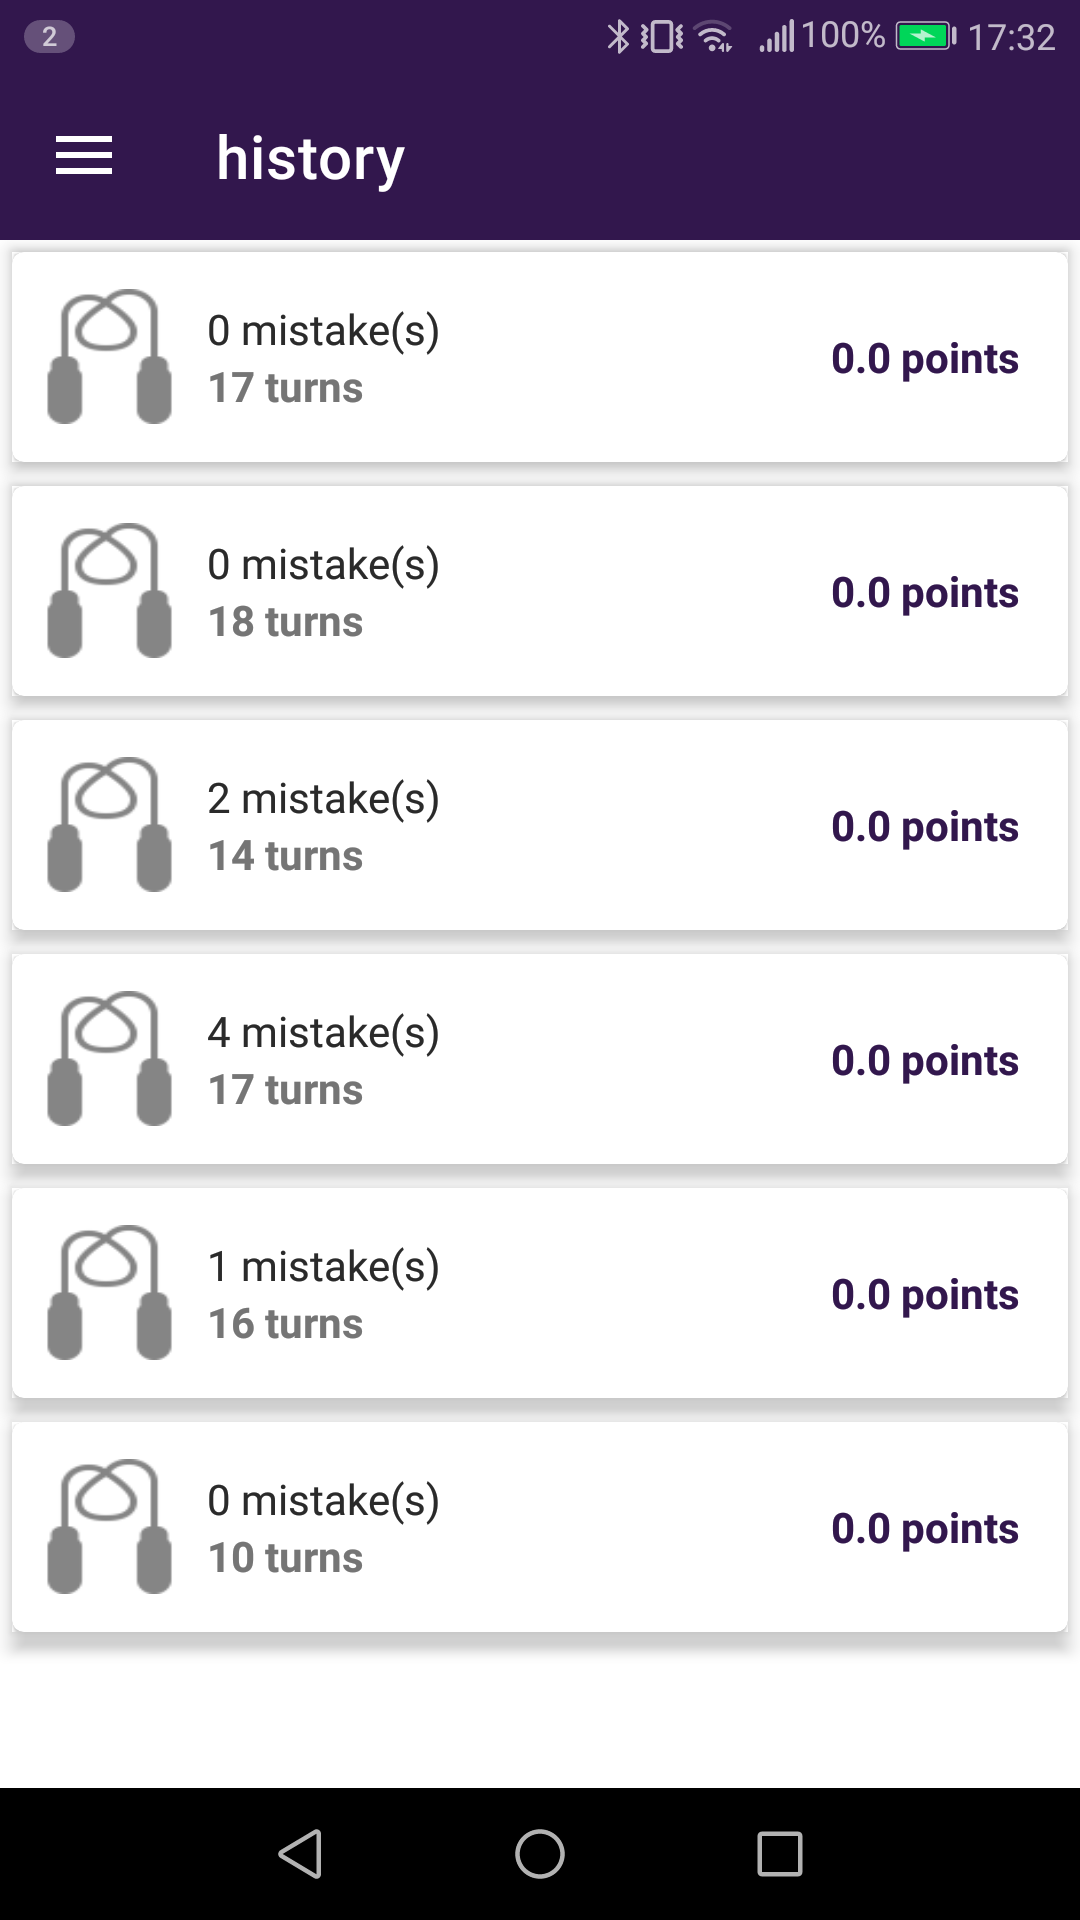
\includegraphics[width=0.45\textwidth]{gezondheidsapplicatie/history.png} 
\end{figure}

\subsection{Aanbevelingen}
Een eerste proefpersoon met gemiddelde fitheid evalueerde de applicatie gedurende drie dagen. Hierbij werd gefocust op de sprongen side swing en jump fast. Dit werd weerspiegeld in de gegeven aanbevelingen al na de eerste dag. Aangezien de sessies telkens van korte duur waren en hierbij minimale inspanning nodig was, werd het vooropgestelde doel niet gehaald. Dit weerspiegelde zich in het voorgestelde doel voor de volgende dag, wat 51 MET-minuten bedroeg. Dit patroon werd aangehouden gedurende twee additionele dagen. De aanbevelingen pasten zich aan aan de voorkeur van de gebruiker en de gewenste duur (zie Figuur \ref{fig:evaluatie1}).
Een tweede proefpersoon met slechtere conditie evalueerde de applicatie eveneens gedurende drie dagen. De gebruiker was enkel in staat om een side swing uit te voeren. Deze voorkeur weerspiegelde zicht duidelijk in de aanbevelingen (zie Figuur \ref{fig:evaluatie2}). Na de eerste dag zakte het doel met slechts 9 MET-minuten. Dit fenomeen zette zich verder de volgende dagen waarbij geëindigd werd met een doel van 60 MET-minuten. Dit is te verklaren door de hogere leeftijd van deze proefpersoon. Hierdoor wordt sneller een hoge hartslagzone bereikt.

\begin{figure}[!htpd]
\centering
\begin{floatrow}
  \ffigbox[\FBwidth]{\caption{Proefpersoon 1}\label{fig:evaluatie1}}{%
    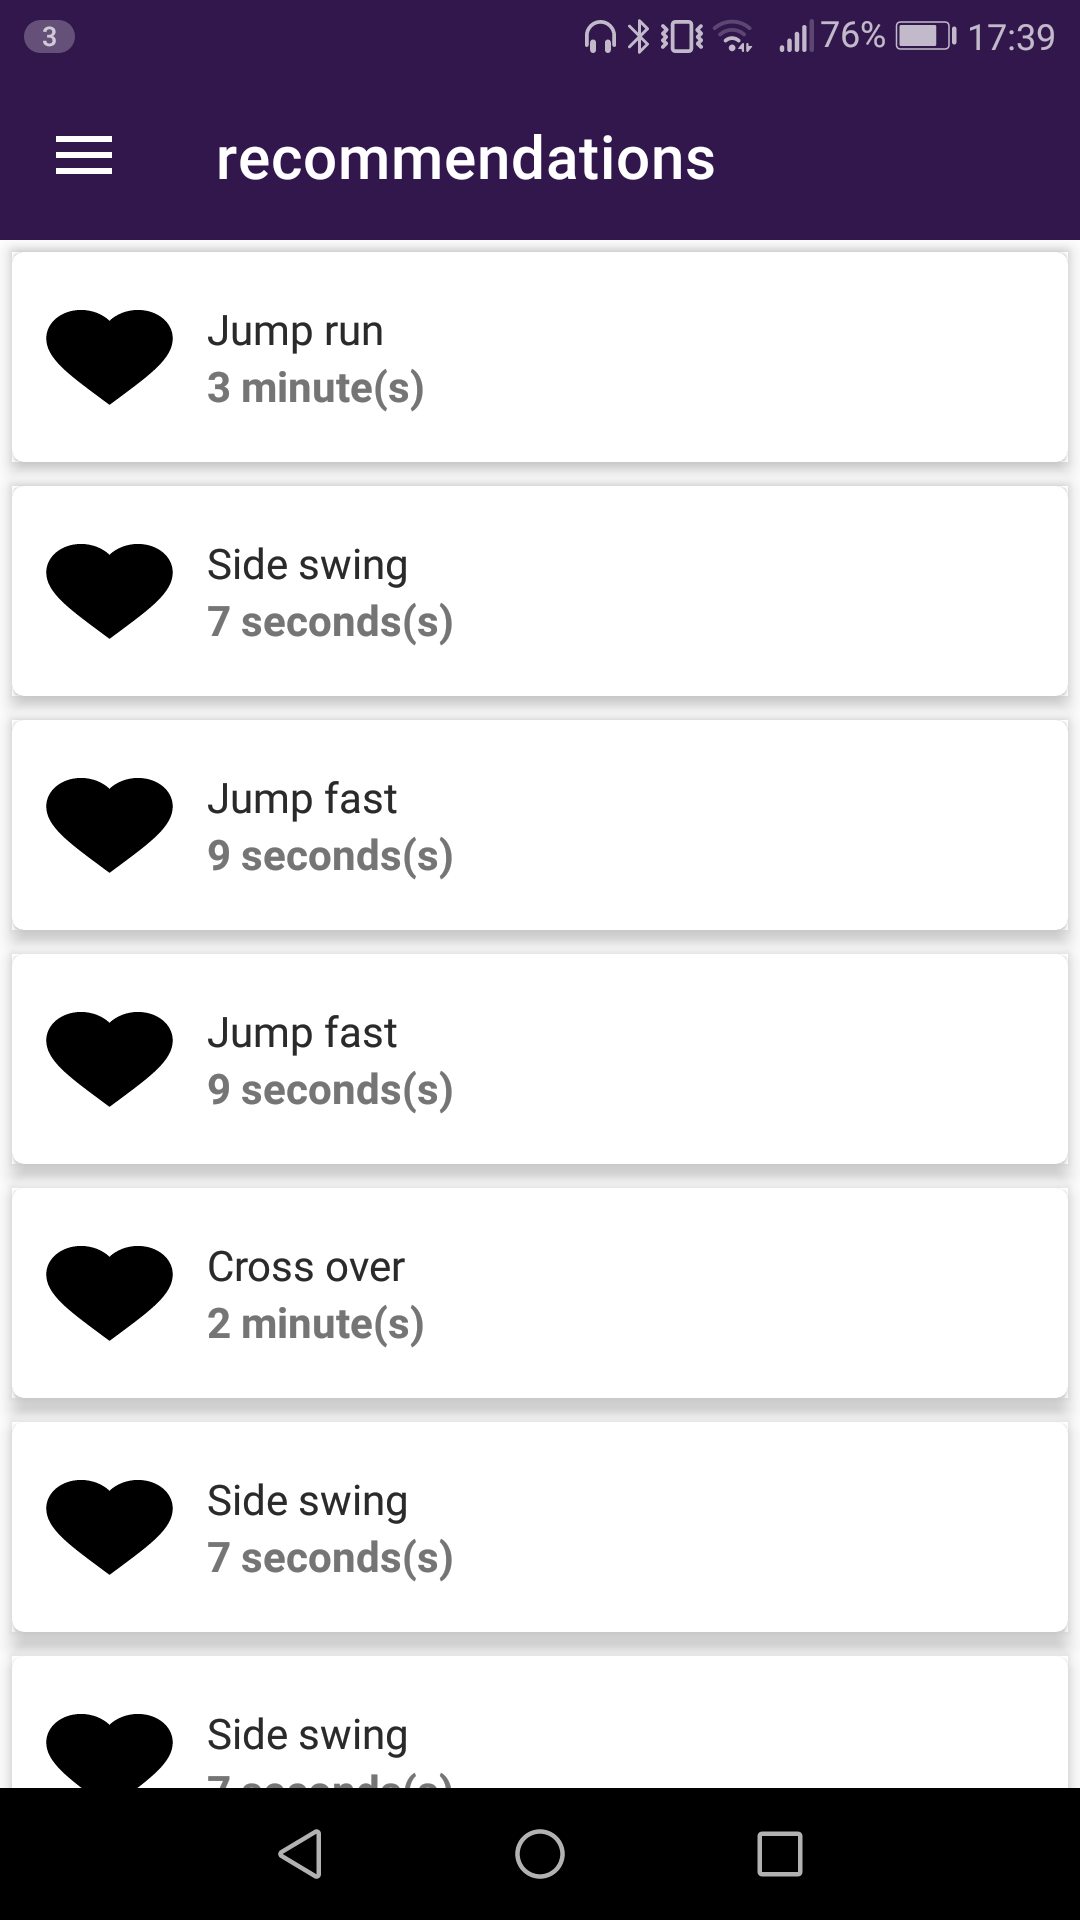
\includegraphics[width=0.45\textwidth]{gezondheidsapplicatie/proefpersoon1_recom.png} 
  }
  \ffigbox[\FBwidth]{\caption{Proefpersoon 2}\label{fig:evaluatie2}}{%
    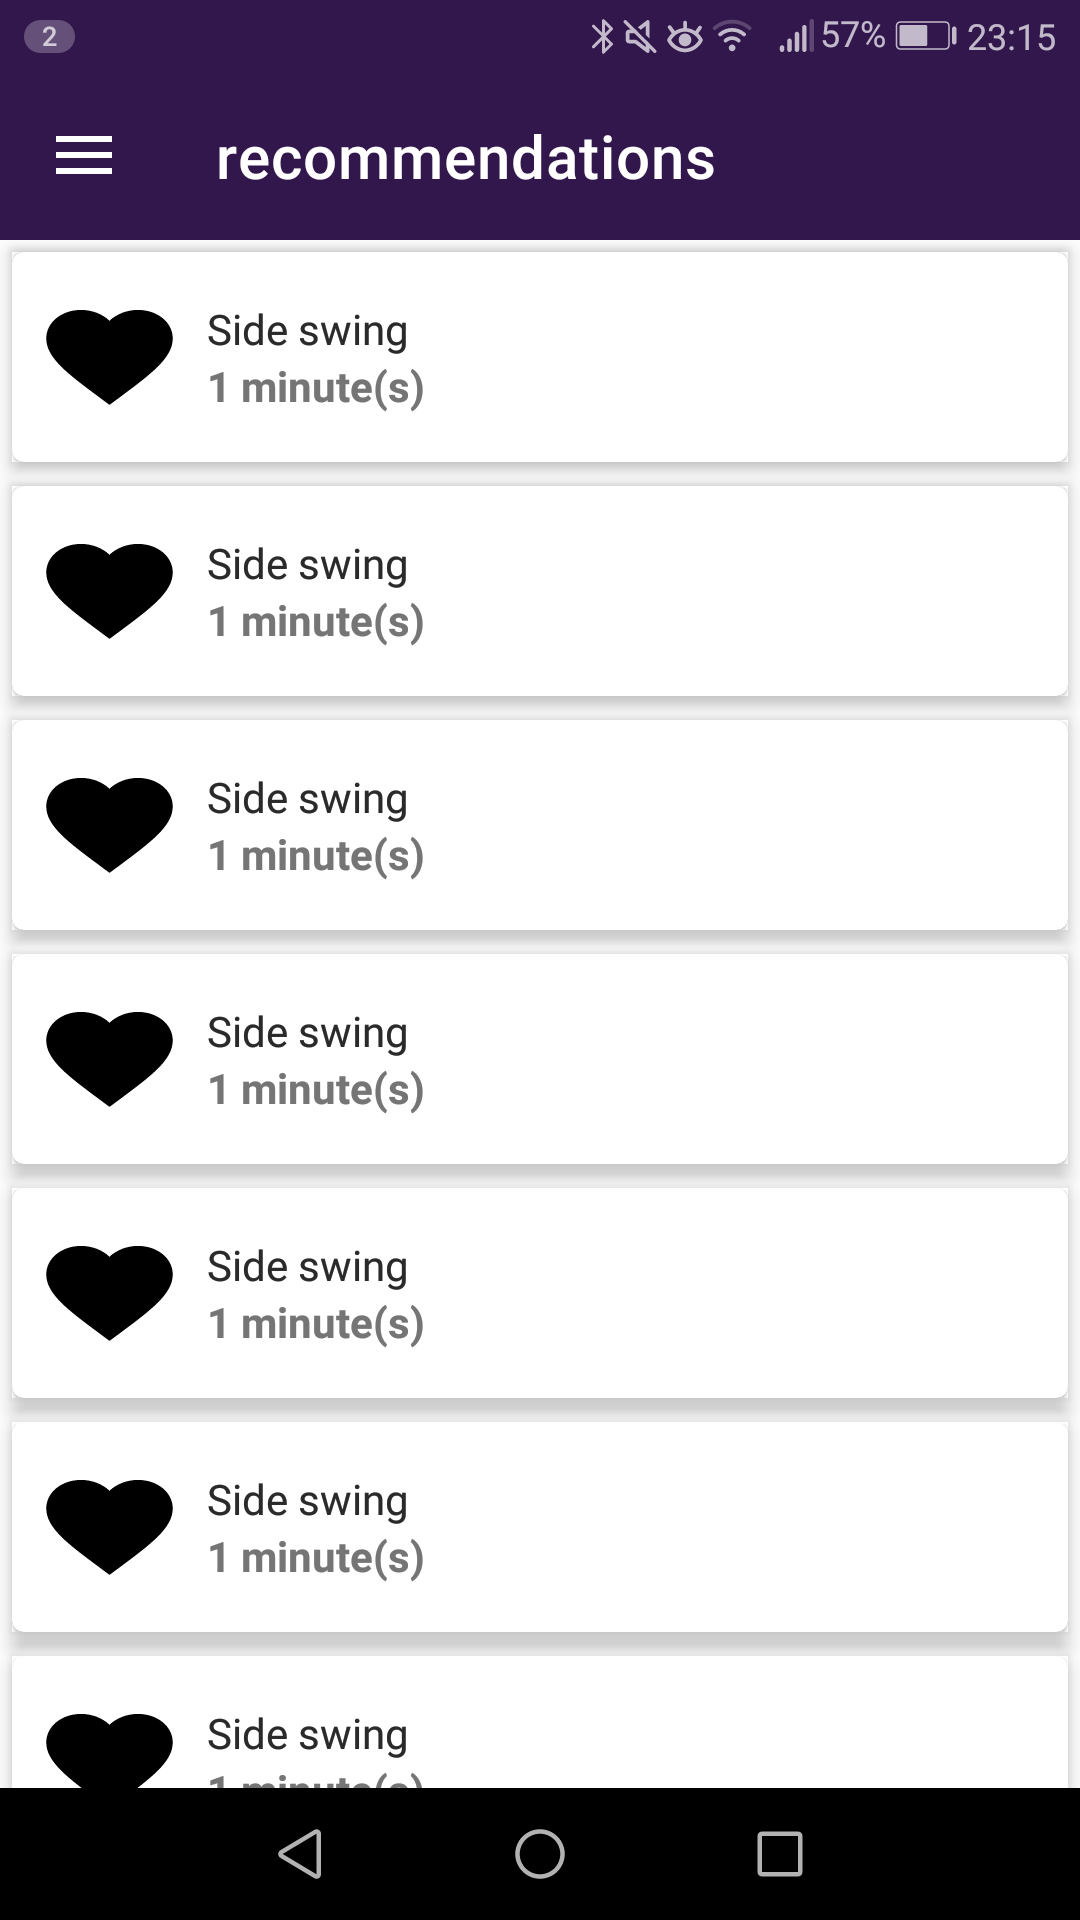
\includegraphics[width=0.45\textwidth]{gezondheidsapplicatie/proefpersoon2_recom.png}
  }
\end{floatrow}
\end{figure}